\documentclass[a4paper,10pt,BCOR=0mm,DIV=14]{scrartcl}

\usepackage[ngerman]{babel}
\usepackage[utf8x]{inputenc}
\usepackage[T1]{fontenc}

\usepackage{csquotes}
\usepackage{graphicx,calc,adjustbox}

\usepackage{hyperref}
\usepackage[noabbrev,ngerman]{cleveref}


\title{Starten der Entdeckerbox-DVD über VirtualBox}

\def\gfxscale{0.27}
\newcommand{\gfxscalebox}[1]{\scalebox{\gfxscale}{#1}}
\newcommand{\smallshadow}[1]{\adjustbox{margin*=-43px -59px -43px  -25px}{#1}}
\newcommand{\command}[1]{\textsf{\enquote{#1}}}

\begin{document}
\maketitle

\section{Einleitung}
Auf der Entdeckerbox-DVD befinden sich nicht nur die einzelnen Programme, Handbücher usw., sondern auch ein Live-System, von dem aus die Programme ohne Installation direkt gestartet werden können. Dazu muss der Computer allerdings heruntergefahren und von der Entdeckerbox-DVD neu gestartet (\enquote{gebootet}) werden.

Dies ist -- auch aus Sicherheitsgründen -- nicht überall möglich. Hier bietet eine virtuelle Maschine Abhilfe: Ein Programm simuliert einen vollständigen \enquote{virtuellen} Computer, auf dem das Entdeckerbox-Live-System ausgeführt wird. Sicherheitsbedenkliche Zugriffe auf den \enquote{echten} Computer bleiben der virtuellen Maschine dabei verwehrt.

In diesem Dokument wird erklärt, wie man so eine virtuelle Maschine mit der kostenlosen, quelloffenen Software Oracle VM VirtualBox erstellt und verwendet.



\section{VirtualBox installieren}
Die Installationsdateien von Oracle VM Virtualbox findest du im \command{IMAGINARY ENTDECKERBOX}-Ordner auf der DVD. Alternativ kannst du auch die jeweils aktuelle Version von Oracle VM VirtualBox auf der Internetseite \url{https://www.virtualbox.org} herunterladen.

Führe das Installationsprogramm für dein Betriebssystem aus und folge dabei den Anweisungen. Nach dem Start von VirtualBox sollte das Programm etwa wie in \cref{VBox10} aussehen. Bitte beachte, dass sich die folgenden Anweisungen und \nameCrefs{VBox10} je nach Betriebssystem geringfügig unterscheiden können.

\begin{figure}[h!]
\centering \gfxscalebox{\smallshadow{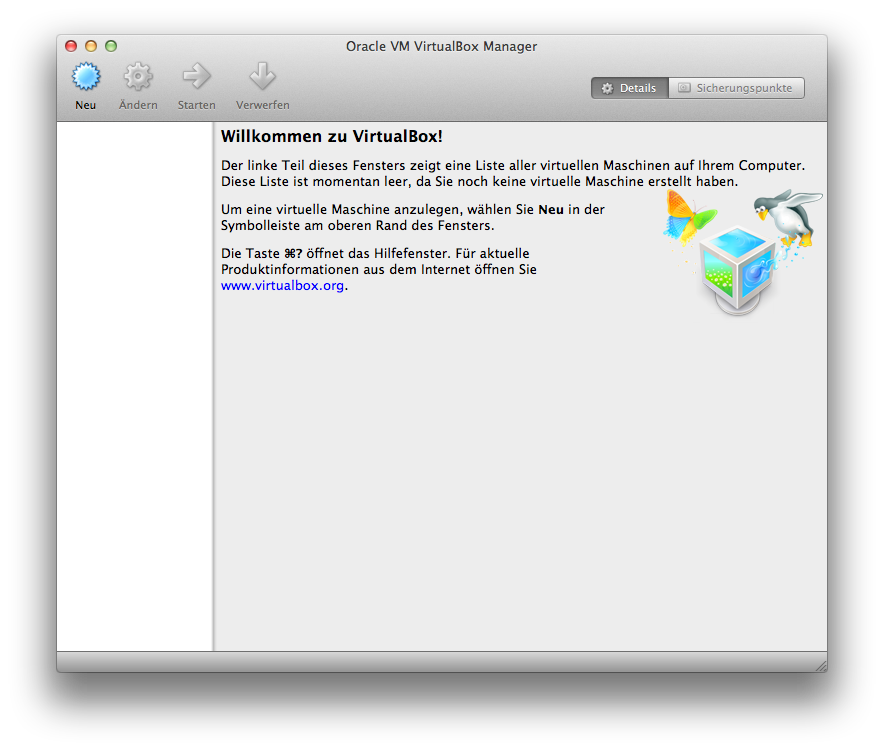
\includegraphics{VBox10}}}
\caption{Startbildschirm von Oracle VM VirtualBox.}
\label{VBox10}
\end{figure}

\section{Eine virtuelle Maschine anlegen}
Um nun eine virtuelle Maschine anzulegen, klickt man in VirtualBox of \command{Neu}. Im folgenden Dialog gibt man der virtuellen Maschine einen Namen, z.\,B. \command{IMAGINARY Entdeckerbox} und wählt Typ (\command{Linux}) und Version (\command{Ubuntu (64\, bit)}) des Systems aus, welches später ausgeführt werden soll. Als nächstes stelle man die Größe des Arbeitsspeichers ein, der der virtuellen Maschine zugewiesen werden soll. Hierbei sollte mindestens 1\, GB gewählt werden. Etwas mehr kann aber auch nicht schaden. Der nächste Schritt wäre das Anlegen einer virtuellen Festplatte. Da wir aber von DVD starten wollen, können wir hier \command{Keine Festplatte} auswählen und bestätigen. Jetzt erscheint die frisch erstellte virtuelle Maschine in der Liste auf der linken Seite. Den gesamten Vorgang kannst du noch einmal in \cref{VBox20to50} grafisch nachvollziehen.
\begin{figure}[h]
\centering
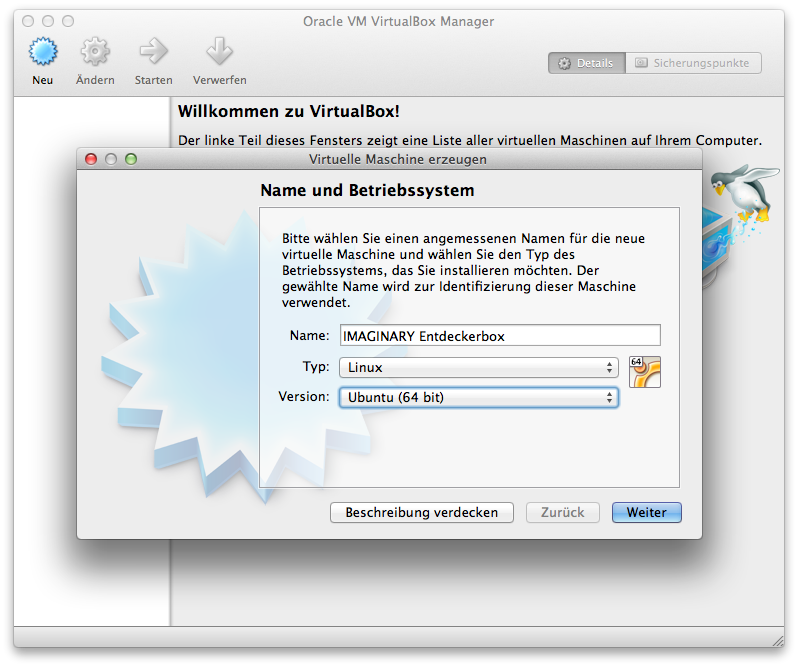
\includegraphics[scale=\gfxscale]{VBox20}
\qquad
\centering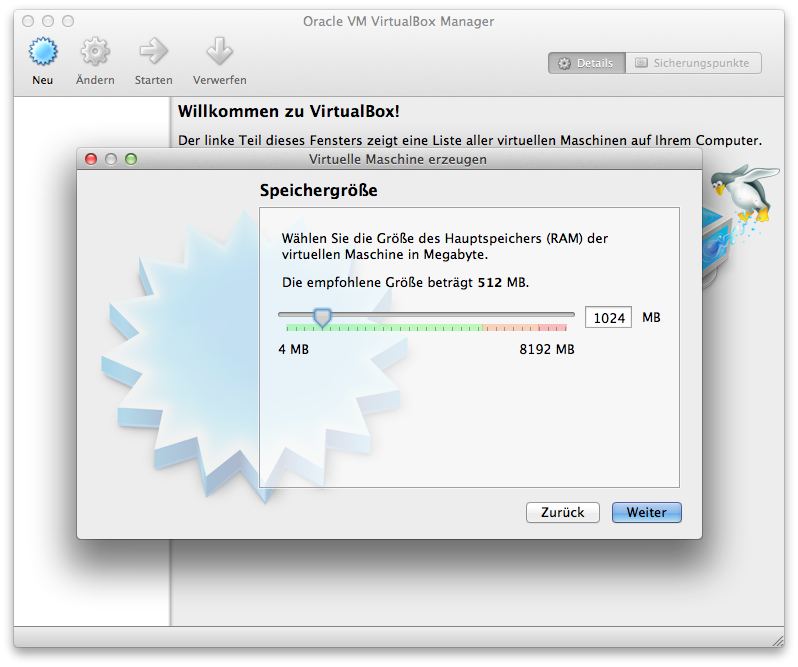
\includegraphics[scale=\gfxscale]{VBox30}
\\[\bigskipamount]
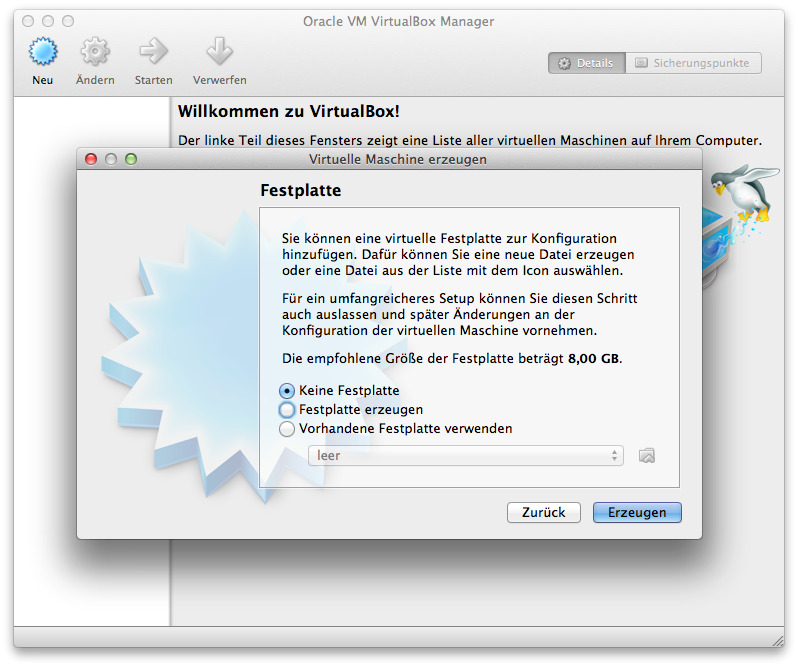
\includegraphics[scale=\gfxscale]{VBox40}
\qquad
\centering\gfxscalebox{\smallshadow{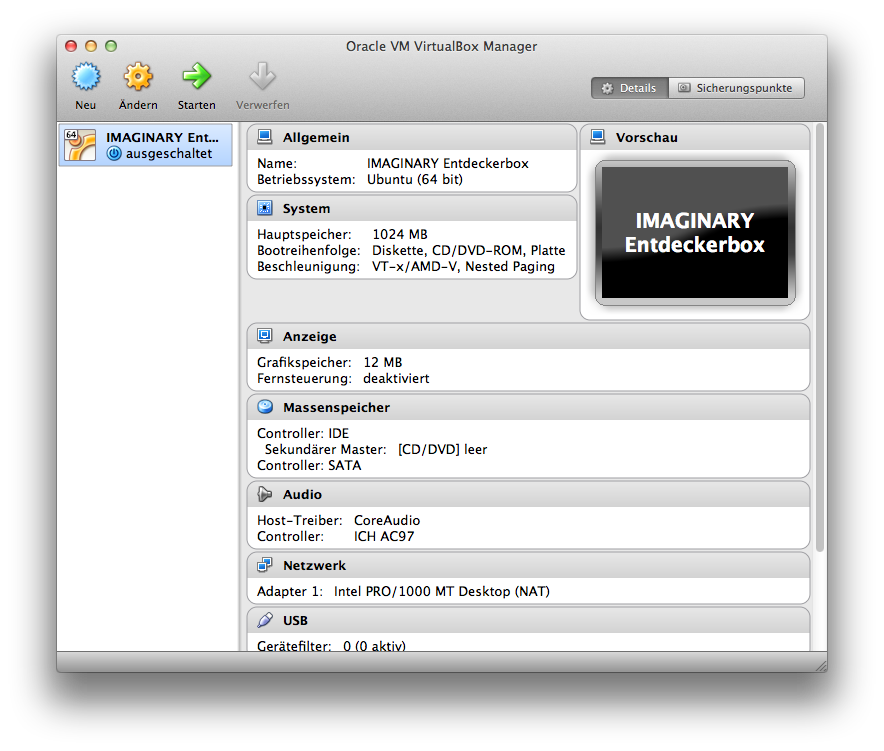
\includegraphics{VBox50}}}
\caption{Schritte zum Anlegen der virtuellen Maschine.}
\label{VBox20to50}
\end{figure}

Da einige Programme der Live-DVD sehr aufwendige Berechnungen durchführen, empfiehlt es sich der virtuellen Maschine noch etwas mehr Rechenpower zur Verfügung zu stellen. Wähle hierzu die \command{IMAGINARY Entdeckerbox}-Maschine aus der Liste aus und klicke auf \command{Ändern}. Unter \command{System} $\rightarrow$ \command{Prozessor} kann man festlegen, wie viele Prozessoren (\command{CPUs}) deines Computers die virtuelle Maschine verwenden darf. Innerhalb des grünen Bereichs sollte der Wert hier möglichst hoch eingestellt sein. In \cref{VBox60} wurden also 8 der 16 verfügbaren Prozessoren ausgewählt. Ein Wert innerhalb des roten Bereichs kann in manchen Fällen kontraproduktiv sein. Wer möchte, kann ein wenig mit den Einstellungen experimentieren um die optimale Leistung zu erzielen. Die Einstellungen für die Grafikkarte befinden sich unter \command{Anzeige}. Hier sollte man etwas Grafikspeicher für die virtuelle Maschine reservieren und die 3D-Beschleunigung aktivieren, etwa so wie in \cref{VBox60} gezeigt.
\begin{figure}[h]
\centering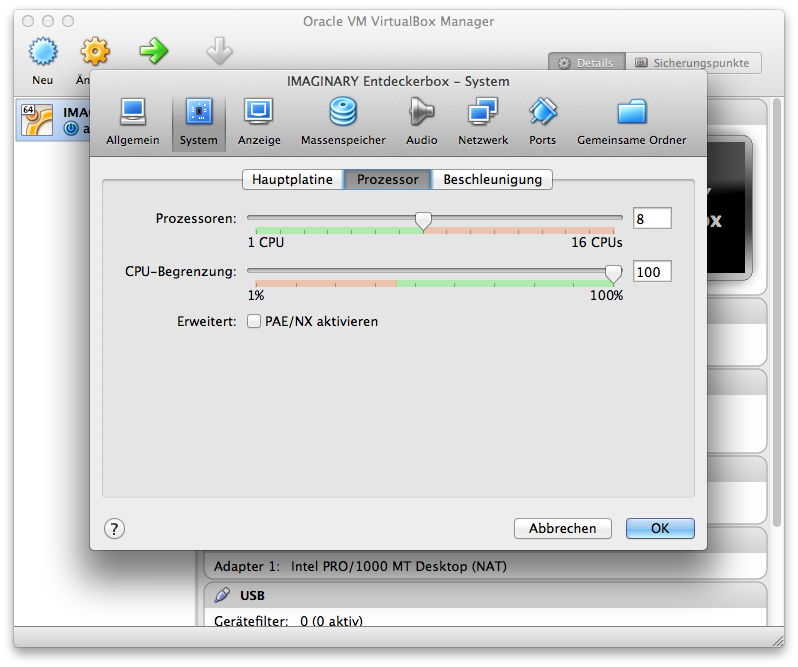
\includegraphics[scale=\gfxscale]{VBox60}
\qquad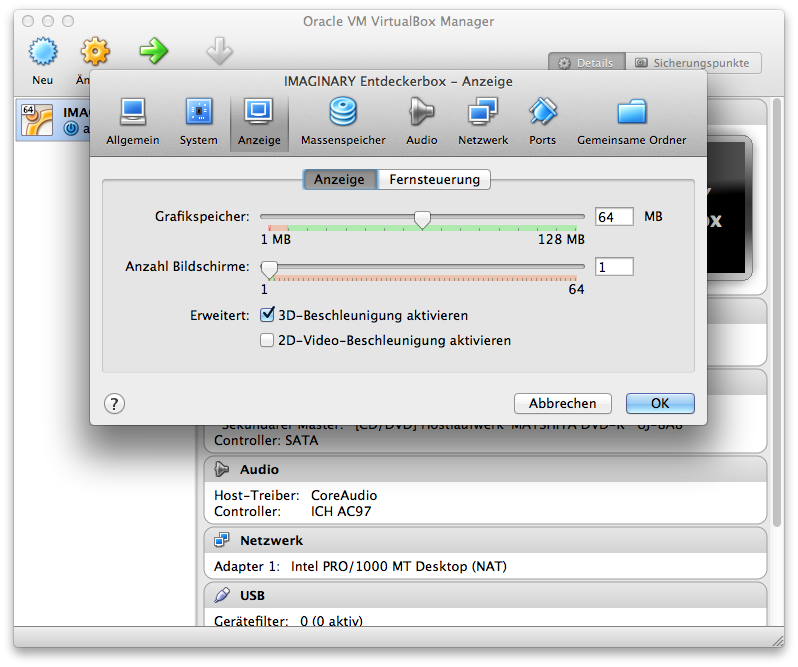
\includegraphics[scale=\gfxscale]{VBox61}
\caption{Der virtuellen Maschine sollten etwa 50\% der tatsächlich vorhanden Prozessoren zugewiesen werden. Auch der Grafikspeicher sollte etwas erhöht und die 3D-Beschleunigung aktiviert werden.}
\label{VBox60}
\end{figure}

\section{Die Entdeckerbox Live-DVD starten}
Bevor du die virtuelle Maschine starten kannst, musst du noch sicherstellen, dass dafür auch wirklich die Entdeckerbox-DVD verwendet wird. Das virtuelle DVD-Laufwerk von VirtualBox soll also auf die Entdeckerbox-DVD in dem realen DVD-Laufwerk deines Computers zugreifen. Dies kannst du unter \command{Ändern} $\rightarrow$ \command{Massenspeicher} wie in \cref{VBox70} beschrieben einstellen. Bitte beachte, dass der Name deines DVD-Laufwerks, der hinter \command{Hostlaufwerk} erscheint, wahrscheinlich anders lautet als in der \namecref{VBox70}. Setze nun noch den Haken bei \command{Live-CD/DVD} und beende das Dialogfenster mit \command{OK}.
\begin{figure}[h]
\centering\scalebox{\gfxscale}{\hspace{312px}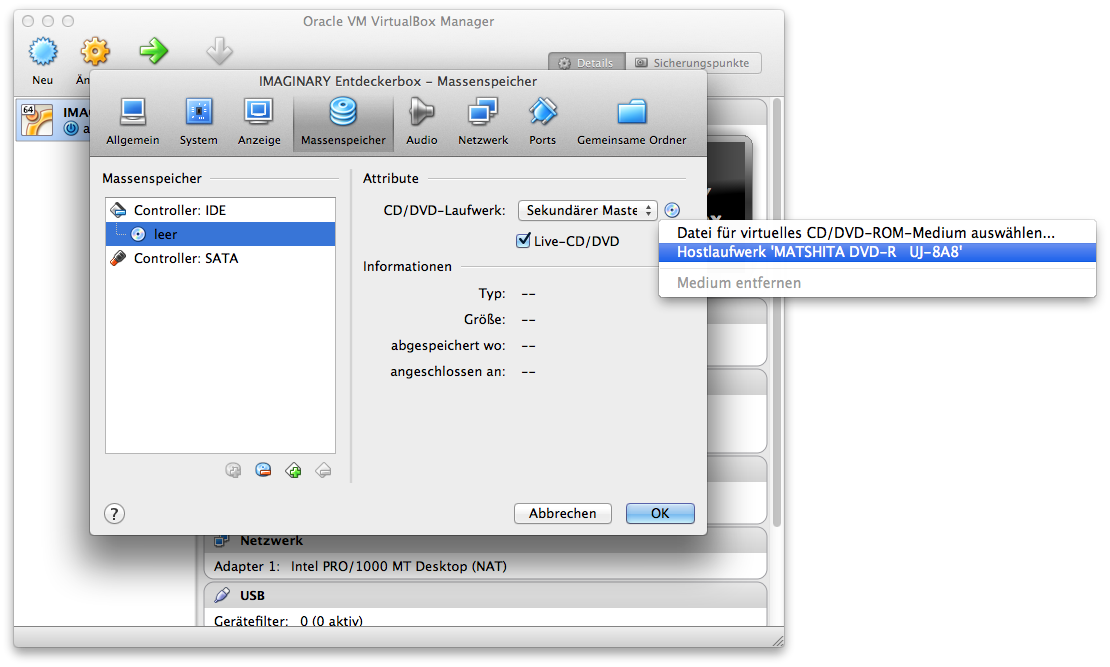
\includegraphics{VBox70}}
\caption{Einlegen der Entdeckerbox-DVD in das virtuelle DVD-Laufwerk.}
\label{VBox70}
\end{figure}

Gratulation! Damit sind alle Einstellungen der virtuellen Maschine erledigt und es kann losgehen. Ein Klick auf den grünen \command{Starten}-Pfeil fährt das System hoch. Das sollte etwa so aussehen wie in \cref{VBox8090}.

Wie du siehst, läuft die Live-DVD nun im Fenstermodus. Im Menü der laufenden virtuellen Maschine kann man unter \command{Ansicht} (engl. \command{View}) auf \command{Vollbild} (engl. \command{Fullscreen}) umschalten. Da die Programme auf der Entdeckerbox-DVD nicht automatisch auf diese Umstellung reagieren, müssen sie jeweils neu gestartet werden. Im Entdeckerbox-Menü kann man z.\,B. einfach \command{ESC} drücken. Danach sollte die Auflösung stimmen.

\begin{figure}[h]
\centering
\gfxscalebox{\smallshadow{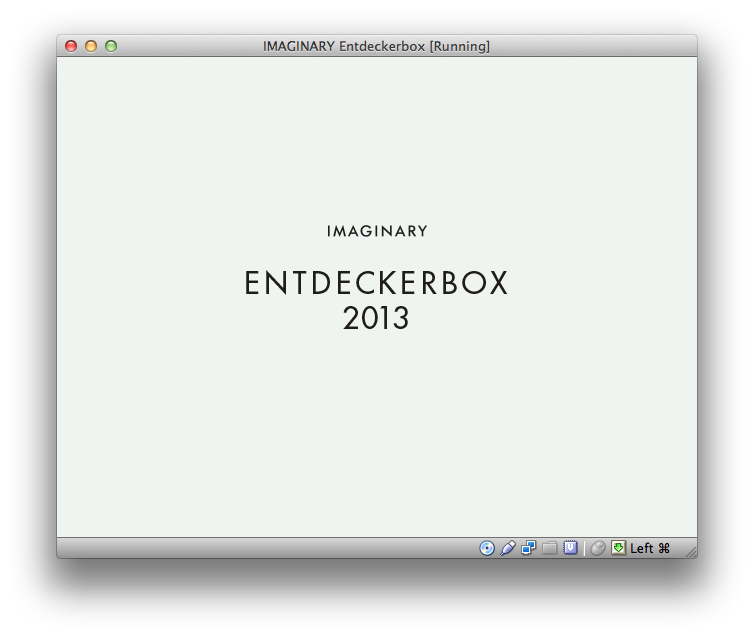
\includegraphics{VBox80}}}
\qquad
\gfxscalebox{\smallshadow{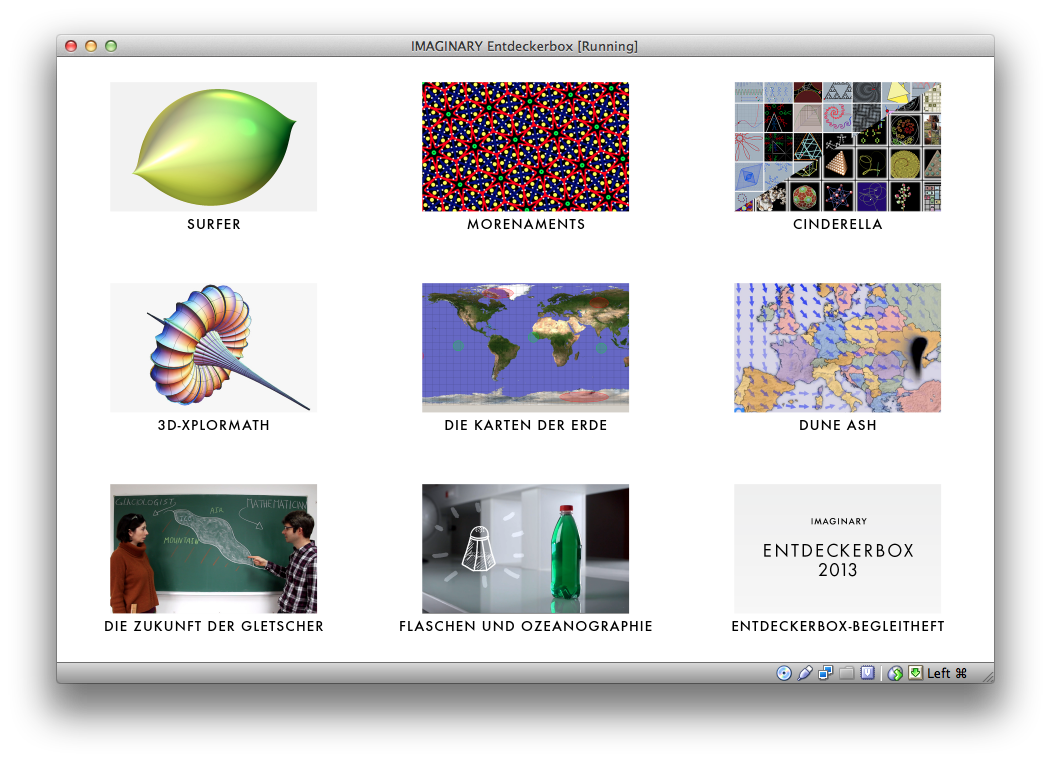
\includegraphics{VBox90}}}
\caption{Nach dem Hochfahren der virtuellen Maschine (links) erscheint nach einiger Zeit das Entdeckerbox-Menü (rechts).}
\label{VBox8090}
\end{figure}

\section{Problembehebung}
\subsection{Ich habe ein 32\,bit Betriebssystem und das Live-System startet nicht!}
Auf der Live-DVD befindet sich ein 64\,bit Betriebssystem. Daher wird ein 64\,bit Prozessor vorausgesetzt. VirtualBox kann auch von deinem 32\,bit Betriebssystem darauf zugreifen. Dafür muss dein Prozessor allerdings die sogenannte Hardware-Virtualisierung unterstützen. Dies trifft für die meisten aktuellen Prozessoren zu, jedoch muss diese Funktion manchmal erst im BIOS aktiviert werden. Die Bezeichnung der Funktion ist je nach Hersteller verschieden (z.\,B. Intel Virtualization Technology, Intel VT-x, Virtualization Extensions, Intel VT-d, AMD-V oder AMD IOMMU). 

\subsection{Das Starten des Live-Systems dauert lange!}
Das Starten eines kompletten Betriebssystems von einer DVD dauert leider eine gewisse Zeit. Man kann die Startzeit erheblich reduzieren, indem man ein ISO-Abbild des Live-Systems auf der Festplatte erstellt. Je nach verwendeter Version des Live-Systems (DVD oder USB-Stick) findest du ein solches Abbild im gleichen Dateiordner wie diese Anleitung oder du musst es selbst erstellen. Die dafür benötigten Programme sind im Internet kostenfrei erhältlich. In einigen Betriebssystemen sind sie bereits enthalten. Wichtig ist in jedem Fall, dass das ISO-Abbild auf einem Datenträger abgelegt wird, der deutlich schneller ist als dein DVD-Laufwerk. Besonders geeignet sind hier Solid-State-Disks.

Das ISO-Abbild wird nun in das virtuelle DVD-Laufwerk gelegt. Dazu musst du im in \cref{VBox70} gezeigten Menü auf \command{Datei für virtuelles CD/DVD-ROM-Medium auswählen} klicken und das ISO-Abbild auswählen.
\end{document} 